\begin{figure}[t]
     \centering
     \begin{subfigure}[b]{0.31\textwidth}
        \centering
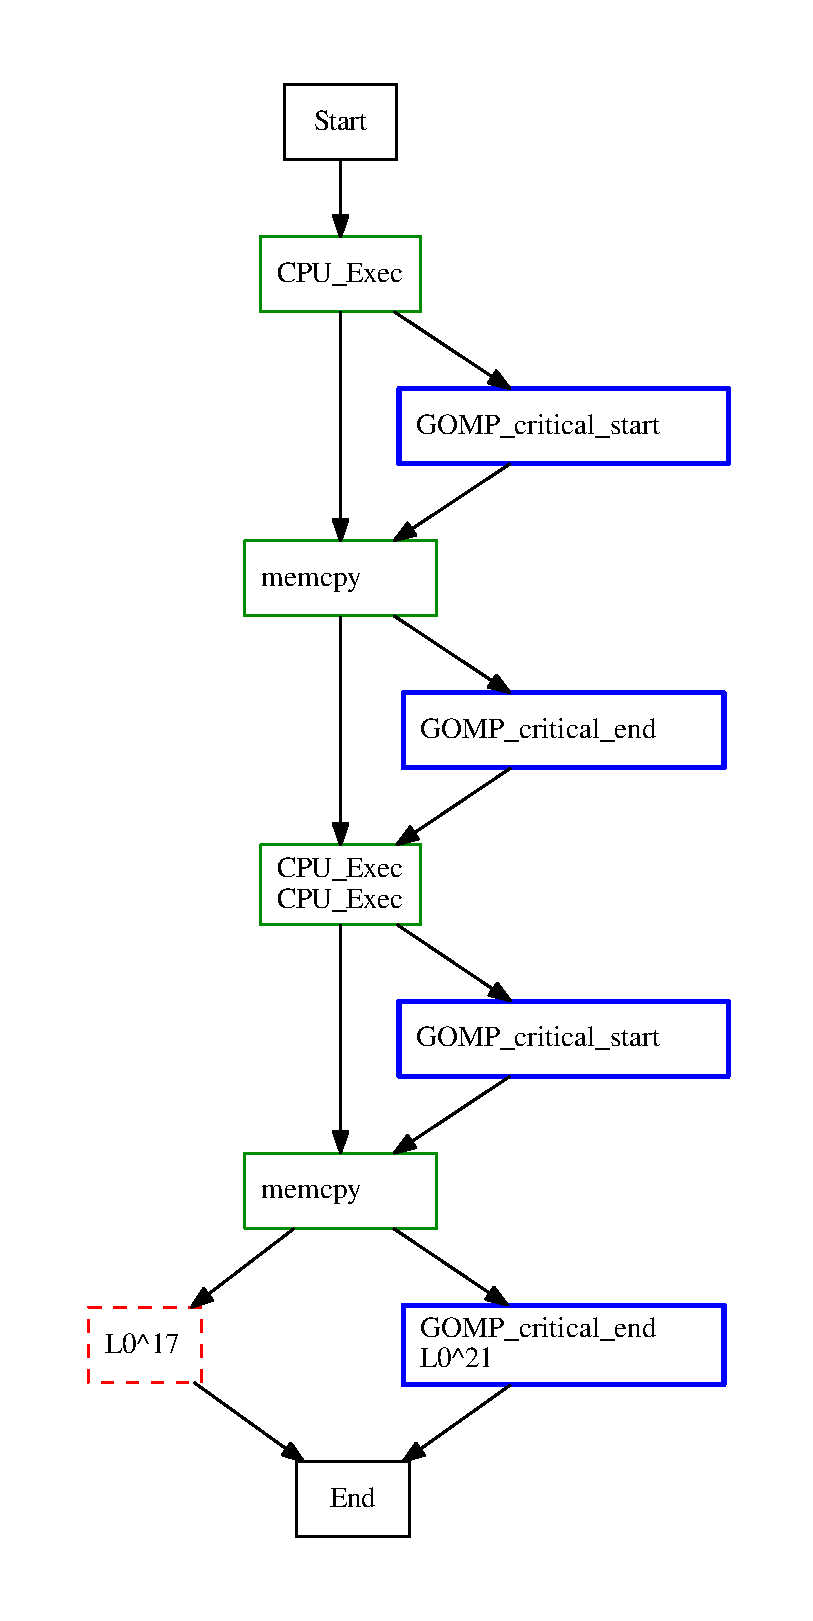
\includegraphics[width=\textwidth]{diffTrace/figs/diffNLR/ompBug-6-4-x0.pdf}
\caption{diffNLR(6.4)}
\label{diffNLR-6-4}
     \end{subfigure}
     \hfill
     \begin{subfigure}[b]{0.31\textwidth}
       \centering
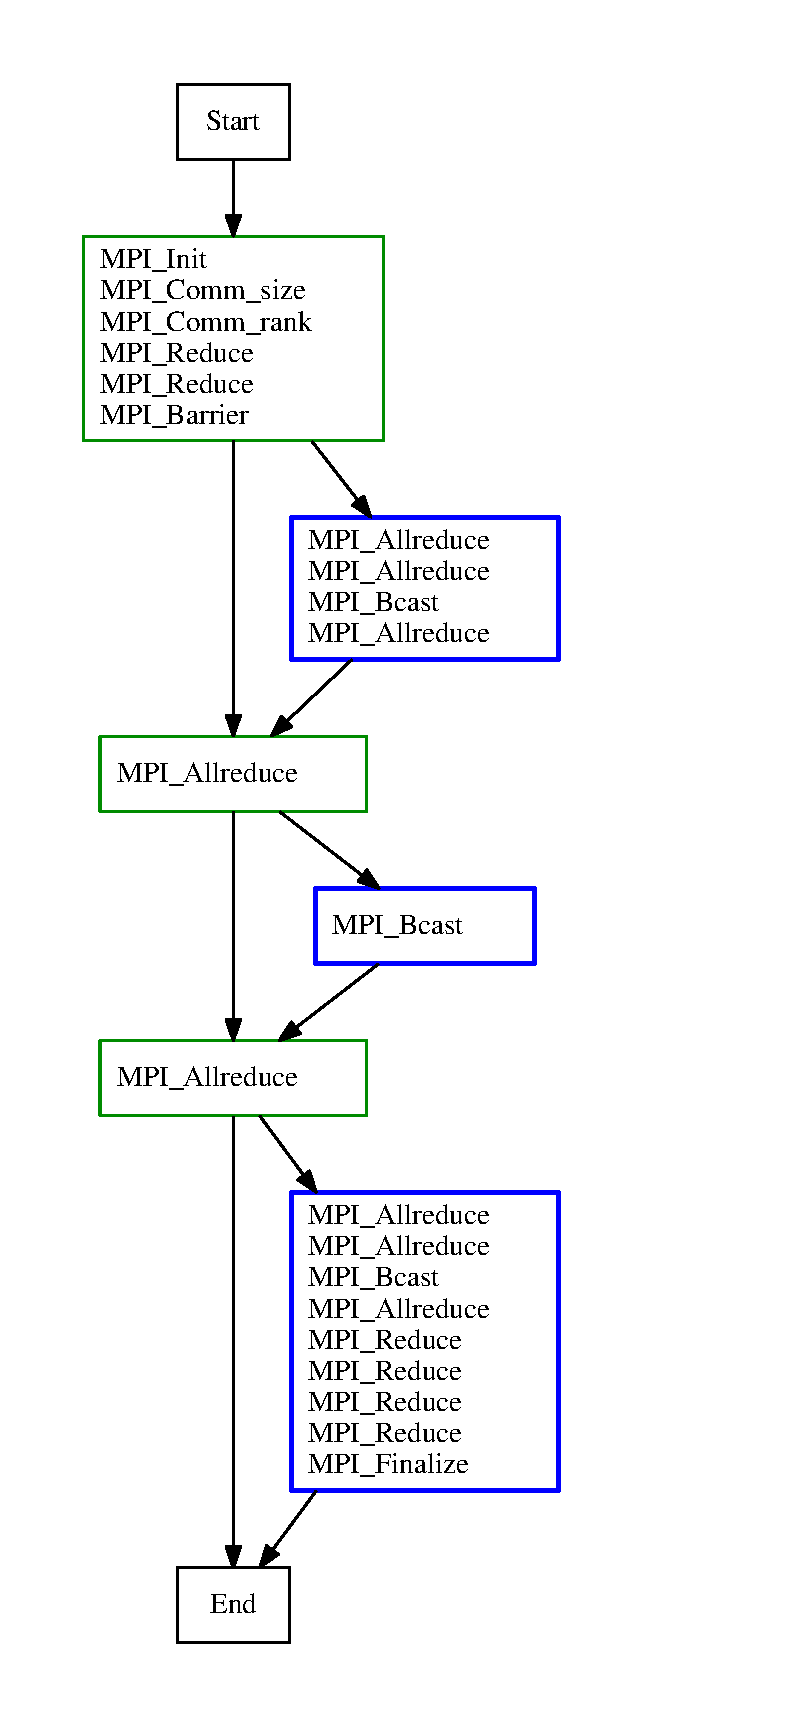
\includegraphics[width=\textwidth]{diffTrace/figs/diffNLR/mpiBug-all-nn-x0.pdf}
\caption{diffNLR(4)}
\label{diffNLR-0}
     \end{subfigure}
     \hfill
     \begin{subfigure}[b]{0.31\textwidth}
         \centering
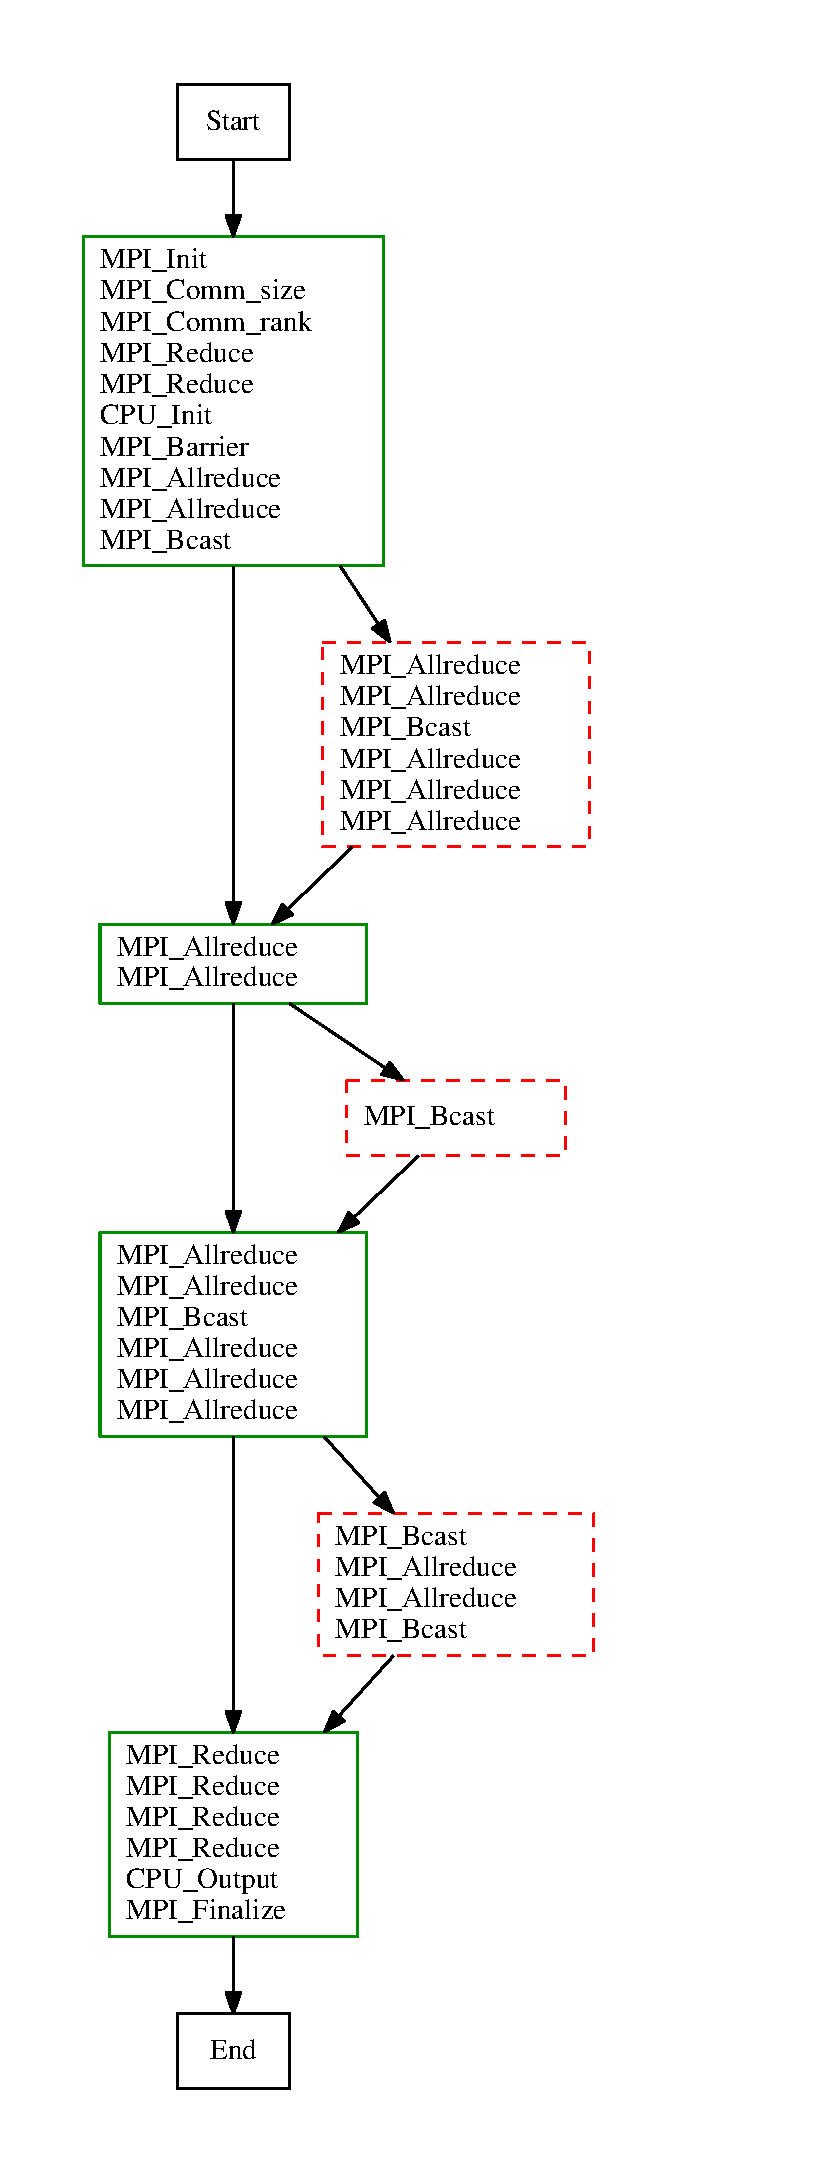
\includegraphics[width=0.9\textwidth]{diffTrace/figs/diffNLR/mpiBug2-0-nn-x0.pdf}
\caption{diffNLR(5)}
\label{diffNLR-5}
     \end{subfigure}
        \caption{Three diffNLR outputs}
        \label{fig:three graphs}
\end{figure}



ILCS is a scalable framework for running iterative local searches on HPC platforms~\cite{ilcs}.
%
Providing serial CPU and/or single-GPU code, ILCS executes this code in parallel between compute nodes (MPI) and within them (OpenMP and CUDA).
%

To evaluate DiffTrace, we manually injected MPI-level and OMP-level bugs into the Traveling Salesman Problem (TSP) running on ILCS (Listing~\ref{lst:ilcs}).
%
The injected bugs simulate real HPC bugs such as deadlocks.
%
%These bugs are close to common mistakes that HPC developers usually make during developing HPC codes.
%
Moreover, we inserted ``hidden'' faults that do not crash the program such as violations of critical sections and semantic bugs.
%
%The injected bugs are planted in a way that might get triggered in only one or more threads (master and worker threads, one thread, every other thread, all threads except one, all threads).
%
The goal was to see how effectively DiffTrace can analyze the resulting traces and how close it can get to the root cause of the fault.
%


%
We collected ParLOT (main image) traces from the execution of ILCS-TSP with 8 MPI processes and 4 OpenMP threads per process on the XSEDE-PSC Bridges supercomputer whose compute nodes have 128 GB of main memory and contain 2 Intel Haswell (E5-2695 v3) CPUs with 14 cores each running at 2.3 - 3.3 GHz.
%
Note that we did not provide any GPU code to ILCS.
%

The collected traces (faulty and normal) are fed to DiffTrace. We enabled the MPI, OpenMP, and custom (ILCS-TSP user code) filters and set the NLR constant K to 10 for all experiments.
%
The current version of DiffTrace is implemented and built using C++ GCC 5.5.0, Pin 3.8, Python 2.7, and Scipy 1.3.0.

%
We present the results in the form of ranking tables that show which traces (processes and threads) DiffTrace considers ``suspicious''. Since DiffTrace output is highly dependent to ``parameters'', each row in ranking tables starts with parameters whom the suspicious traces are the result of.

The linkage method that converts JSMs to flat clustering is ``ward'' for all of the top reported suspicious traces that we removed from tables for better readability. Ward linkage function in SciPy uses \textit{Ward variance minimization algorithm} to calculate the distance between newly formed clusters~\cite{scipy}. Furthermore, we show diffNLRs for selected traces.



\subsection{ILCS-TSP Workflow}

The TSP code starts with a random tour and iteratively shortens it using the 2-opt improvement heuristic~\cite{2-opt} until a local minimum is reached. ILCS automatically and asynchronously distributes unique seed values to each worker thread, runs the TSP code, reduces the results to find the best solution, and repeats these steps until the termination criterion is met. It employs two types of threads per node: a \textit{master} thread (MPI process) that handles the communication and local work distribution and a set of \textit{worker} threads (OpenMP threads) that execute the provided TSP code. The master thread forks a worker thread for each detected CPU core.
%
Each worker thread continually calls
\texttt{CPU\_Exec()} to evaluate a seed and records the result (lines 14-20).
%
Once the worker threads are running, the master thread's primary job is to scan the results of the workers to find the best solution computed so far (i.e., the local champion). This information is then globally reduced to determine the current system-wide champion (lines 22-32).
%
ILCS terminates the search when the quality has not improved over a certain period (lines 33-34).



\subsection{OpenMP Bug: Unprotected Memory Access}

The memory accesses performed by the \texttt{memcpy} calls on lines 20 and 30 are protected by an OpenMP critical section.
%
Not protecting them results in a data race that might lead to incorrect final program output.
%
To simulate this scenario, we modified the ILCS source code to omit the critical section in worker thread 4 of process 6.

Table~\ref{tab:mc1-mc-6-4} lists the top suspicious traces that DiffTrace finds when injecting this bug.
%
Each row presents the results for different filters and attributes.
%
For example, the filter ``11.mem.ompcit.cust.0K10'' removes all function returns and .plt calls from the traces and only keeps memory-related calls, OpenMP critical-section functions, and the custom function ``CPU\_Exec''.
%
The ``K10'' at the end of filter means that the filtered traces are converted into an NLR with $K$=10.
%
%\hl{I will remove two unnecessary columns from the tables (threshold and linkage function) to save space and add 2-3 sentences explaining what was them}
%
The bold numbers in the rightmost column of the table flag trace 6.4 (i.e., process 6, thread 4) as the trace that was affected the most by the bug.
%

The corresponding diffNLR(6.4) presented in Figure~\ref{diffNLR-6-4} clearly shows that the normal execution of ILCS (green and blue blocks) protects the \texttt{memcpy} while the buggy execution (green and red blocks) does not. Here, L0 represents \texttt{CPU\_Exec}, which is called multiple times in both the fault-free and the buggy version (the call frequencies are different due to the asynchronous nature of ILCS).
%


%\begin{figure}[]
%\centering
%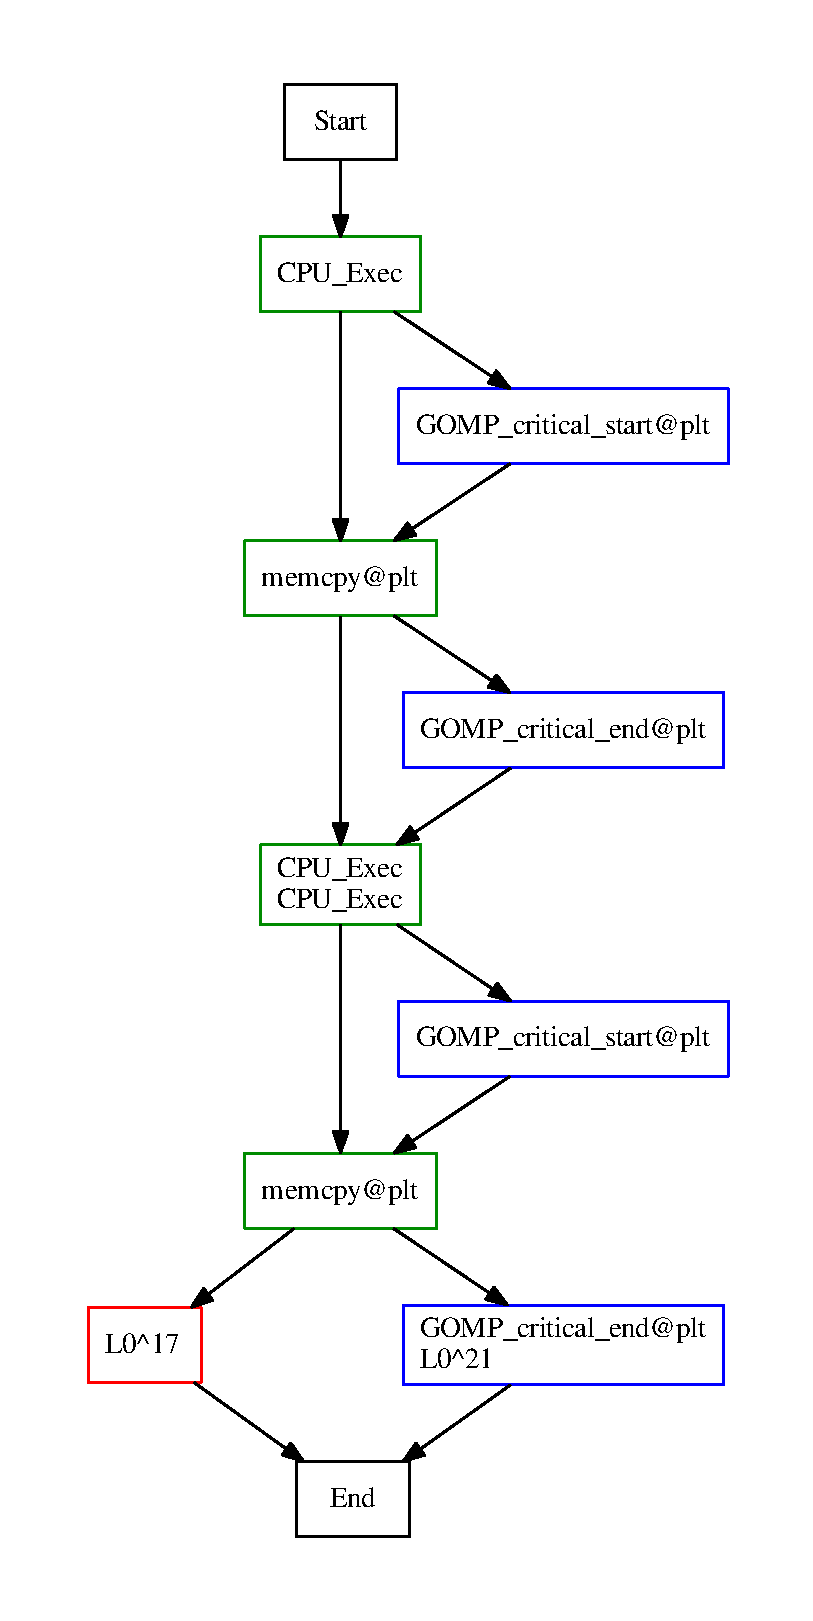
\includegraphics[width=0.3\textwidth]{figs/diffNLR/ompBug-6-4.pdf}
%\caption{OpenMP Bug: diffNLR(6.4)}
%\label{diffNLR-6-4}
%\end{figure}


\subsection{MPI Bug: Deadlock Caused by Fault in Collective}

By forcing process 2 to invoke MPI\_Allreduce (line 24) with a wrong size, we can inject a \textit{real deadlock}.
%
Because the deadlock happens early in the execution, the resulting traces are very different from their fault-free counterparts.
%
Consequently, DiffTrace marks almost all processes as suspicious (cf.~Table~\ref{tab:ar1-ws-all-nn}).
%
Clearly, this is not helpful for debugging.
%
Nevertheless, diffNLR still yields useful information.
%
Since most of the traces are suspicious, we do not know which one the real culprit is and randomly selected trace~4.
%
%It turned out that ParLoT did not happen to capture function calls from all processes since the bug happens too early in the code. Thus except for process 1 and 4, all other traces are empty.
%
By looking at the diffNLR(4) output shown in Figure~\ref{diffNLR-0}, we immediately see that both the normal and the buggy trace are identical up to the invocation of MPI\_Allreduce. This gives the user the first (correct) hint as to where the problem lies.
%
Beyond this point, the bug-free process continues to the end of the program
(it reaches the MPI\_Finalize call) whereas the buggy process does not. The last entry in the buggy trace is a call to MPI\_Allreduce (the last green box), indicating that this call never returned, that is, it deadlocked. This provides the user with the second (correct) hint as to the type of the underlying bug.
%

%
\begin{table}[b]
\centering
\caption{Ranking table - MPI bug: wrong collective size in process 2}
\label{tab:ar1-ws-all-nn}
\scalebox{0.81}{
\begin{tabular}{|c|c|c|c|c|}
\hline
 Filter              & Attributes   &    B-score & \begin{tabular}[c]{@{}c@{}}Top\\Processes\end{tabular}          & \begin{tabular}[c]{@{}c@{}}Top\\Threads\end{tabular}         \\
\hline
% 11.mem.mpicol.ompcrit.cust.0K10 & sing.log10   &      0.383 & 0 , 7 , 2 , 4 , 5 , 6 , & 1.1 , 1.3 , 1.4 , 3.1 , 3.2 , 3.4 , \\
% 11.mem.mpicol.ompcrit.cust.0K10 & sing.noFreq  &      0.383 & 0 , 7 , 2 , 4 , 5 , 6 , & 1.1 , 1.3 , 1.4 , 3.1 , 3.2 , 3.4 , \\
 11.mpicol.cust.0K10             & sing.log10   &      0.439 & 0, 7, 2, 4, 5, 6  & 1.1, 1.3, 3.1, 3.2, 3.4        \\
 11.mpicol.cust.0K10             & sing.noFreq  &      0.439 & 0, 7, 2, 4, 5, 6  & 1.1, 1.3, 3.1, 3.2, 3.4        \\
 11.mpi.cust.0K10                & doub.noFreq  &      0.457 & 0, 7, 2, 4, 5, 6  & 1.4, 3.3, 3.4                    \\
 11.mpi.cust.0K10                & doub.actual  &      0.457 & 0, 7, 2, 4, 5, 6  & 1.4, 3.3, 3.4                    \\
 11.mpiall.cust.0K10             & doub.noFreq  &      0.457 & 0, 7, 2, 4, 5, 6  & 1.4, 3.3, 3.4                    \\
 11.mpiall.cust.0K10             & doub.actual  &      0.457 & 0, 7, 2, 4, 5, 6  & 1.4, 3.3, 3.4                    \\
 11.mpicol.cust.0K10             & doub.noFreq  &      0.457 & 0, 7, 2, 4, 5, 6  & 1.4, 3.3, 3.4                    \\
 11.mpicol.cust.0K10             & doub.actual  &      0.457 & 0, 7, 2, 4, 5, 6  & 1.4, 3.3, 3.4                    \\
 11.mpi.cust.0K10                & sing.log10   &      0.465 & 0, 7, 2, 4, 5, 6  & 1.1, 1.3, 3.1, 3.2, 3.4        \\
 11.mpi.cust.0K10                & sing.noFreq  &      0.465 & 0, 7, 2, 4, 5, 6  & 1.1, 1.3, 3.1, 3.2, 3.4        \\
 11.mpiall.cust.0K10             & sing.log10   &      0.465 & 0, 7, 2, 4, 5, 6  & 1.1, 1.3, 3.1, 3.2, 3.4        \\
 11.mpiall.cust.0K10             & sing.noFreq  &      0.465 & 0, 7, 2, 4, 5, 6  & 1.1, 1.3, 3.1, 3.2, 3.4        \\
 11.mpi.cust.0K10                & doub.noFreq  &      0.543 & 0, 7, 2, 4, 5, 6  & 1.4, 3.3, 3.4                    \\
 11.mpi.cust.0K10                & doub.actual  &      0.543 & 0, 7, 2, 4, 5, 6  & 1.4, 3.3, 3.4                    \\
\hline
\end{tabular}}
\end{table}


%\begin{figure}[]
%\centering
%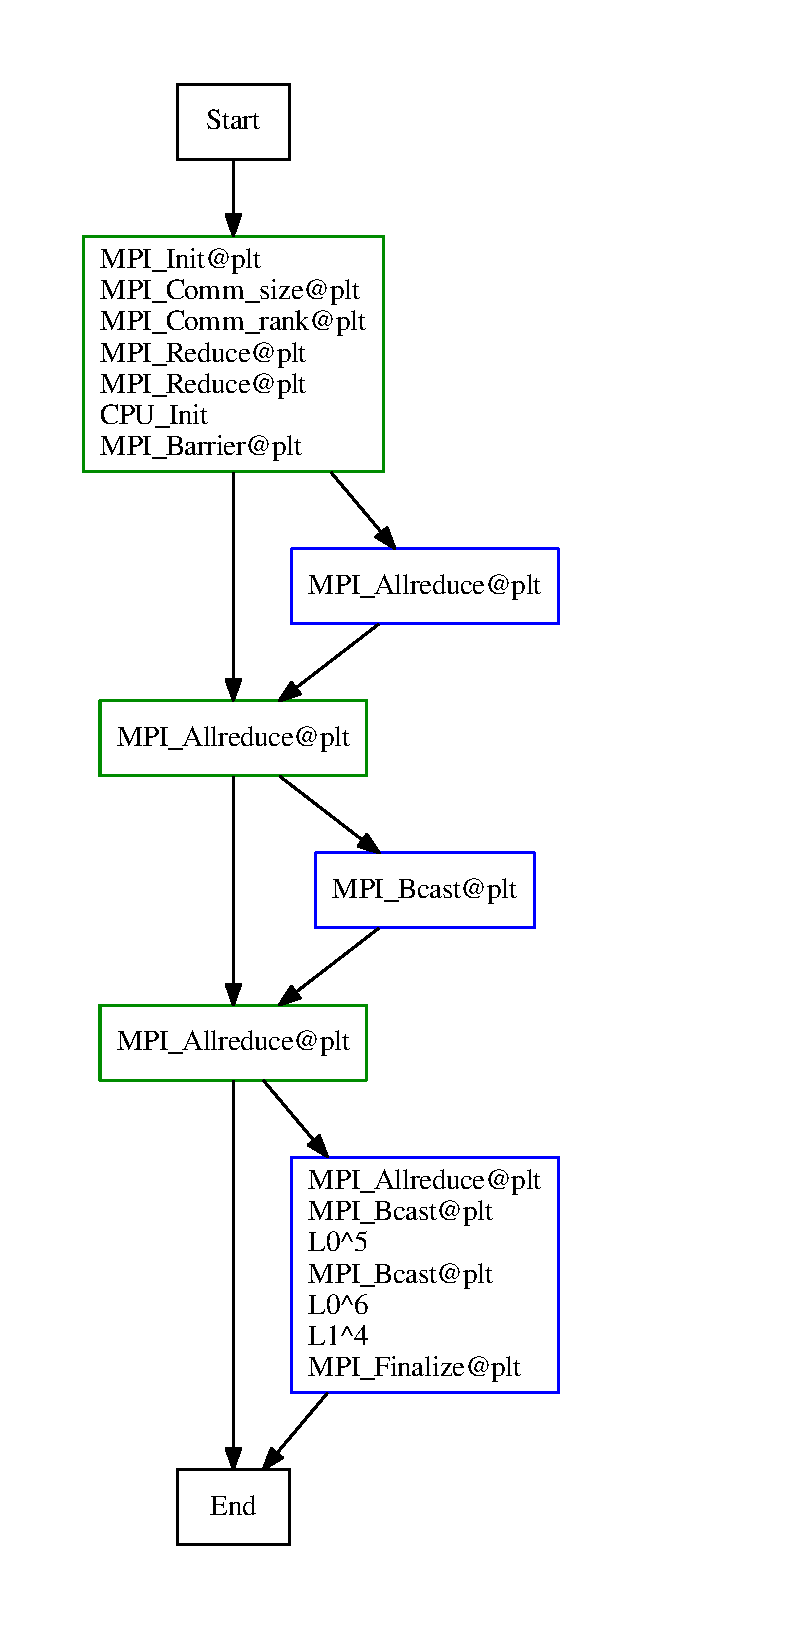
\includegraphics[width=0.3\textwidth]{figs/diffNLR/mpiBug-all-nn.pdf}
%\caption{diffNLR(0)}
%\label{diffNLR-0}
%\end{figure}
%





\subsection{MPI Bug: Wrong Collective Operation}

By changing the MPI\_MIN argument to MPI\_MAX in the MPI\_Allreduce call on line 24 of Listing~\ref{lst:ilcs}, the semantics of ILCS change.
%
Instead of computing the best answer, the modified code computes the worst answer.
%
Hence, this code variation terminates but is likely to yield the wrong result.
%
We injected this bug into process 0.

The first few suspicious processes listed in Table~\ref{tab:ar1-wo-0-nn} are inconclusive. However, the filters that include MPI all agree that process 5 changed the most.
%
Looking at the corresponding diffNLR(5) output in Figure~\ref{diffNLR-5} makes it clear why process 5 was singled out. In the buggy run, it executes many more MPI\_Bcast calls than in the bug-free run because the frequency in which local ``optimums'' are produced has changed. Though this should affect all traces equally, which has reflected in the diffNLR of other traces. We are presenting these tables and figures to show that DiffTrace can reveal the impact of silent bugs like the wrong operation. Such data representation via suggested tables and diffNLRs helps developers to gain insight into the general behavior of the execution. More accurate results can be obtained by refining the parameters and collecting more profound traces (e.g., ParLOT(all images)). This would be part of our future work to find the set of parameters for different classes of bugs to maximize accuracy.



%\begin{figure}[]
%\centering
%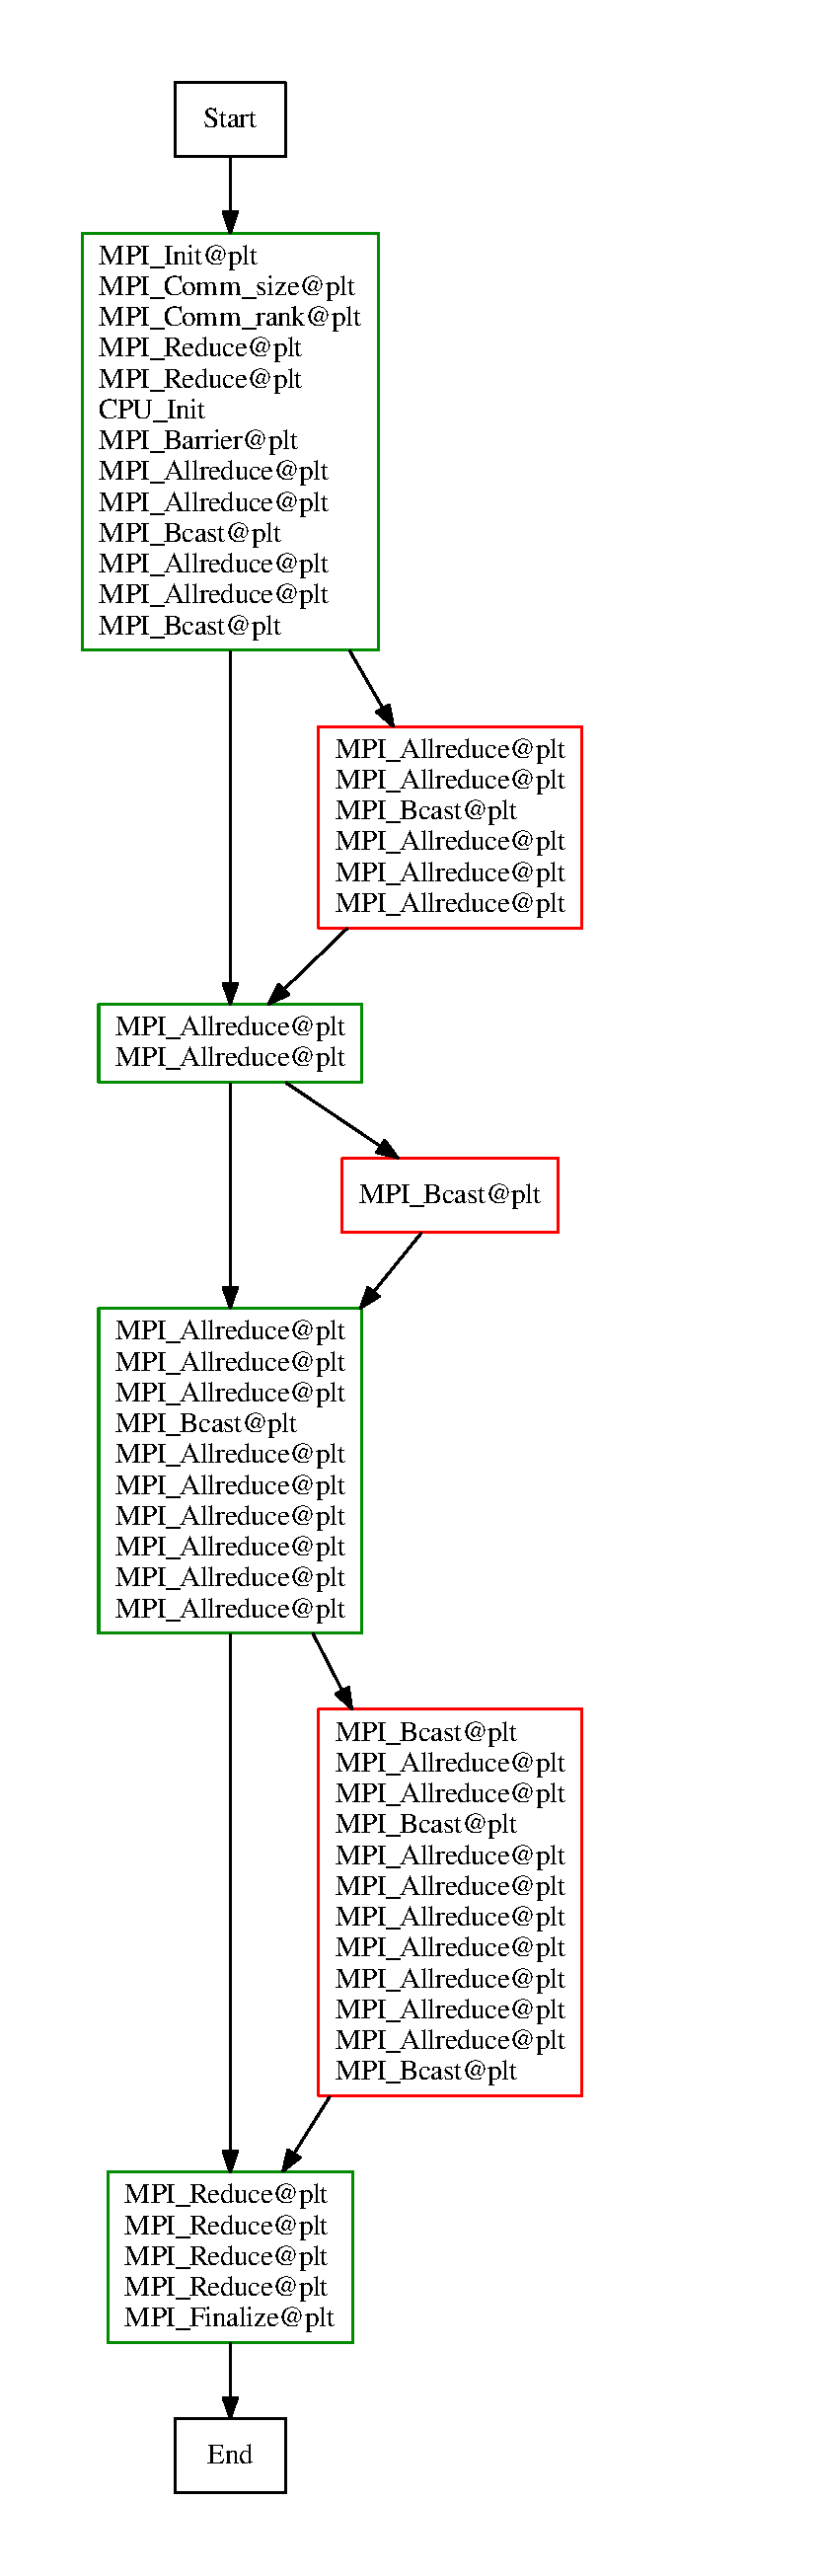
\includegraphics[width=0.3\textwidth]{figs/diffNLR/mpiBug2-0-nn.pdf}
%\caption{diffNLR(5)}
%\label{diffNLR-5}
%\end{figure}
